\documentclass{article}
\usepackage[margin=1in]{geometry}
\usepackage{amsmath,amsthm,amssymb}
\usepackage{bbm,enumerate,mathtools}
\usepackage{tikz,pgfplots}
\usepackage{chessboard}
\usepackage[hidelinks]{hyperref}
\usepackage{multicol} % Problem 35
\usepackage{xstring} % Difficulty command
\usetikzlibrary{shapes.geometric}

\newenvironment{question}{\begin{trivlist}\item[\textbf{Question.}]}{\end{trivlist}}
\newenvironment{note}{\begin{trivlist}\item[\textbf{Note.}]}{\end{trivlist}}
\newenvironment{references}{\begin{trivlist}\item[\textbf{References.}]}{\end{trivlist}}
\newenvironment{related}{\begin{trivlist}\item[\textbf{Related.}]\end{trivlist}\begin{enumerate}}{\end{enumerate}}

\newcommand\score[1]{
\pgfmathsetmacro\pgfxa{#1+1}
\tikzstyle{scorestars}=[
  star,
  star points=5,
  star point ratio=2.25,
  draw,
  inner sep=3pt,
  anchor=outer point 5
]
  \begin{tikzpicture}[baseline]
    \draw[opacity=0] (0,-0.5) rectangle (0,0.2); % Workaround for whitespace at the bottom.
    \foreach \i in {1,...,4} {
      \pgfmathparse{(\i<=#1?"yellow":"gray")}
      \edef\starcolor{\pgfmathresult}
      \draw (\i*4.5ex,0) node[name=star\i,scorestars,fill=\starcolor]  {};
    }
  \end{tikzpicture}
}

\newcommand{\difficulty}[1]{%
  \IfEqCase{#1}{%
      {1}{
        
\begin{tikzpicture}[scale=0.7, baseline=0.9mm]%
          \definecolor{slopegreen}{rgb}{0.0, 0.5, 0.0}%
          \fill[slopegreen] (0.5,0.5) circle (0.5);%
        \end{tikzpicture}%
      }%
      {2}{
        
\begin{tikzpicture}[scale=0.7, baseline=0.9mm]%
          \definecolor{slopeblue}{rgb}{0.0, 0.44, 1.00}
          \fill[slopeblue] (0,0) rectangle (1,1);%
        \end{tikzpicture}%
      }%
      {3}{
\begin{tikzpicture}[scale=0.7, baseline=0.9mm]\fill (0,0.5)--(0.5, 0)--(1,0.5)--(0.5,1)--cycle; \end{tikzpicture}}%
      {4}{
\begin{tikzpicture}[scale=0.7, baseline=0.9mm]\fill (0.25,0)--(0,0.5)--(0.25,1)--(0.5,0.5)--cycle; \fill (0.75,0)--(0.5,0.5)--(0.75,1)--(1,0.5)--cycle;\end{tikzpicture}}%
      % you can add more cases here as desired
  }[\PackageError{difficulty}{Undefined difficulty level: #1}{}]%
}%
\newcommand{\rating}[2]{\difficulty{#1}\\\score{#2}\\}


\begin{document}
  Consider integer functions $f$ from an $n$-element subset of $\mathbb{N}$
  such that no $k$ of the points
  $\{(j_1, f(j_1)),\hdots,(j_n, f(j_n))\}$ fall on a $k-2$-degree polynomial.

\begin{figure}[!h]
  \centering
  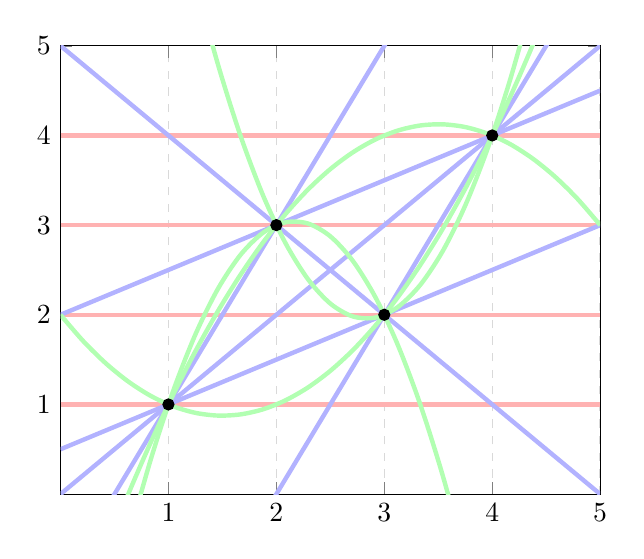
\begin{tikzpicture}[scale=1]
    \begin{axis}[
      xmin=0, xmax=5,
      ymin=0, ymax=5,
      domain=0:5,
      grid=both,
      grid style={line width=0.5pt, draw=gray!30, dashed},
      ytick={1,...,7},
      xtick={1,...,7},
      smooth
    ]
      \addplot[red!30, ultra thick] (x,1);
      \addplot[red!30, ultra thick] (x,2);
      \addplot[red!30, ultra thick] (x,3);
      \addplot[red!30, ultra thick] (x,4);

      \addplot[blue!30, ultra thick] (x,2*x-1);

      \addplot[blue!30, ultra thick] (x,x/2+1/2);
      \addplot[blue!30, ultra thick] (x,-x+5);

      \addplot[blue!30, ultra thick] (x,x);
      \addplot[blue!30, ultra thick] (x,2 + x/2);
      \addplot[blue!30, ultra thick] (x,-4 + 2*x);

      \addplot[green!30, ultra thick] (x,-3*x^2/2 + 13*x/2 - 4);
      \addplot[green!30, ultra thick] (x,-x^2/2 + 7*x/2 - 2);
      \addplot[green!30, ultra thick] (x,x^2/2 - 3*x/2 + 2);
      \addplot[green!30, ultra thick] (x,3*x^2/2 - 17*x/2 + 14);


      \addplot[mark=*] coordinates {(1,1)};
      \addplot[mark=*] coordinates {(2,3)};
      \addplot[mark=*] coordinates {(3,2)};
      \addplot[mark=*] coordinates {(4,4)};
    \end{axis}
  \end{tikzpicture}
  \caption{
    An example that shows that $a(4) = 4$.
    (Degree 0 polynomials are plotted in red, degree 1 in blue, and degree 2 in green.)
  }
\end{figure}

\begin{question}
  What is $a(n)$, the least $N$ such that there exists a function
  $f\colon \{ 1,2,\hdots,n \} \rightarrow \{ 1,2,\hdots,N \}$
  with the above property?
\end{question}

\begin{note}
  Trivially, $a(n)$ is bounded above by the function described in problem 23.
\end{note}

\begin{related}
  \item What is the least $M$ such that there exists a subset
  $S \subset \{ 1,2,\hdots,M \}$ and a surjection
  $g\colon S\rightarrow \{ 1,2,\hdots,n \}$ with the aforementioned property?
  \item How many such functions exist when $N$ and $M$ are minimized respectively?
\end{related}
\begin{references}
  \item Problem 23.
\end{references}
\end{document}
